\setcounter{figure}{0}

\section{15th October 2023: I AM the light of the world}
\subsection*{Text: John 8:12-58}
  \begin{quote}
  [12] Again Jesus spoke to them, saying, “I am the light of the world. Whoever follows me will not walk in darkness, but will have the light of life.” [13] So the Pharisees said to him, “You are bearing witness about yourself; your testimony is not true.” [14] Jesus answered, “Even if I do bear witness about myself, my testimony is true, for I know where I came from and where I am going, but you do not know where I come from or where I am going. [15] You judge according to the flesh; I judge no one. [16] Yet even if I do judge, my judgment is true, for it is not I alone who judge, but I and the Father who sent me. [17] In your Law it is written that the testimony of two people is true. [18] I am the one who bears witness about myself, and the Father who sent me bears witness about me.” [19] They said to him therefore, “Where is your Father?” Jesus answered, “You know neither me nor my Father. If you knew me, you would know my Father also.” [20] These words he spoke in the treasury, as he taught in the temple; but no one arrested him, because his hour had not yet come.

  [21] So he said to them again, “I am going away, and you will seek me, and you will die in your sin. Where I am going, you cannot come.” [22] So the Jews said, “Will he kill himself, since he says, ‘Where I am going, you cannot come’?” [23] He said to them, “You are from below; I am from above. You are of this world; I am not of this world. [24] I told you that you would die in your sins, for unless you believe that I am he you will die in your sins.” [25] So they said to him, “Who are you?” Jesus said to them, “Just what I have been telling you from the beginning. [26] I have much to say about you and much to judge, but he who sent me is true, and I declare to the world what I have heard from him.” [27] They did not understand that he had been speaking to them about the Father. [28] So Jesus said to them, “When you have lifted up the Son of Man, then you will know that I am he, and that I do nothing on my own authority, but speak just as the Father taught me. [29] And he who sent me is with me. He has not left me alone, for I always do the things that are pleasing to him.” [30] As he was saying these things, many believed in him.

  [31] So Jesus said to the Jews who had believed him, “If you abide in my word, you are truly my disciples, [32] and you will know the truth, and the truth will set you free.” [33] They answered him, “We are offspring of Abraham and have never been enslaved to anyone. How is it that you say, ‘You will become free’?”

  [34] Jesus answered them, “Truly, truly, I say to you, everyone who practices sin is a slave to sin. [35] The slave does not remain in the house forever; the son remains forever. [36] So if the Son sets you free, you will be free indeed. [37] I know that you are offspring of Abraham; yet you seek to kill me because my word finds no place in you. [38] I speak of what I have seen with my Father, and you do what you have heard from your father.”

  [39] They answered him, “Abraham is our father.” Jesus said to them, “If you were Abraham’s children, you would be doing the works Abraham did, [40] but now you seek to kill me, a man who has told you the truth that I heard from God. This is not what Abraham did. [41] You are doing the works your father did.” They said to him, “We were not born of sexual immorality. We have one Father—even God.” [42] Jesus said to them, “If God were your Father, you would love me, for I came from God and I am here. I came not of my own accord, but he sent me. [43] Why do you not understand what I say? It is because you cannot bear to hear my word. [44] You are of your father the devil, and your will is to do your father’s desires. He was a murderer from the beginning, and does not stand in the truth, because there is no truth in him. When he lies, he speaks out of his own character, for he is a liar and the father of lies. [45] But because I tell the truth, you do not believe me. [46] Which one of you convicts me of sin? If I tell the truth, why do you not believe me? [47] Whoever is of God hears the words of God. The reason why you do not hear them is that you are not of God.”

  [48] The Jews answered him, “Are we not right in saying that you are a Samaritan and have a demon?” [49] Jesus answered, “I do not have a demon, but I honor my Father, and you dishonor me. [50] Yet I do not seek my own glory; there is One who seeks it, and he is the judge. [51] Truly, truly, I say to you, if anyone keeps my word, he will never see death.” [52] The Jews said to him, “Now we know that you have a demon! Abraham died, as did the prophets, yet you say, ‘If anyone keeps my word, he will never taste death.’ [53] Are you greater than our father Abraham, who died? And the prophets died! Who do you make yourself out to be?” [54] Jesus answered, “If I glorify myself, my glory is nothing. It is my Father who glorifies me, of whom you say, ‘He is our God.’ [55] But you have not known him. I know him. If I were to say that I do not know him, I would be a liar like you, but I do know him and I keep his word. [56] Your father Abraham rejoiced that he would see my day. He saw it and was glad.” [57] So the Jews said to him, “You are not yet fifty years old, and have you seen Abraham?” [58] Jesus said to them, “Truly, truly, I say to you, before Abraham was, I am.” [59] So they picked up stones to throw at him, but Jesus hid himself and went out of the temple.
  \end{quote}
\subsection*{Notes}
\begin{itemize}
  \item{The previous “I AM” discourse (bread of life) was given near the passover.}
  \item{The “I AM” discourse for today (light of thr world) was given at the feast of booths. The feast of booths is a Jewish festival celebrating how God tabernacled with the Israelites in the OT and led them by a pillar of cloud by day, and a pillar of fire by night. }
  \item{John chapter 1:9-11 tells us that Jesus is the true light that is rejected by his own. Jesus, the light of the world, has come, but the Jews largely rejected Jesus. But Jesus is not just a light to the Jews, but the light of \textbf{the world}, so Jesus is our light too. }
  \item{Light helps us to see things in darkness. Without light, we become afraid of the dark, we get lost in the dark. Throughout the OT, light has always been how God communicated His presence to the Israelites. See also Exodus 14:19-20.}
  \item{And as per Psalm 27, we see that God is our light and our salvation. And as per Psalm 119, God’s word is a lamp unto our feet and a light onto our path. See also Habbakuk 3:3-4.}
  \item{When Jesus declares himself to he the light of the world, He is just declaring His identity; just like God is our light and our salvation, just like God is the pillar of fire that guided the Israelites, so is Jesus, since Jesus is the Son of God. }
  \item{The darkness of the world is a darkness of sin, ignorance, sorrow and death. Jesus brings forth life and God’s presence, hence He is the light that cuts through the darkness above.}
  \item{The pharisees rejected Jesus’ claim about himself here, since from their POV, Jesus is bearing witness about himself. But Jesus responded that there are actually two witnesses, Jesus and the Father. Jesus testifies about Himself, and the Father testifies about Jesus. And the Father testifies about Jesus through the works that He sends Jesus to do, c.f John 5: 36-19. And as Jesus says in chapter 8, to reject Jesus is to not know both the Father and Jesus (ch 8:19).}
  \item{Jesus’ identity can be captured by the cute acronym LIGHT; Jesus is Lord, Jesus Illuminates, Jesus is God’s Son, Jesus is Hope, and Jesus is Truth.}
  \item{And as Jesus says later on, his claims will be finally vindicated on the cross (ch 8:28-30). For us today, while we don’t see Jesus’ works like feeding the 5000, we see what Jesus did on the cross, we see His death and resurrection, and that vindicates His claims to divinity and Lordship, to being the source of light and eternal life, to being God’s Son, to being our hope, and that He is the truth. Sometimes we forget this, so we need to remember this by looking at the cross.}
  % \item{\begin{figure}[H]
  %   \centering
  %   % 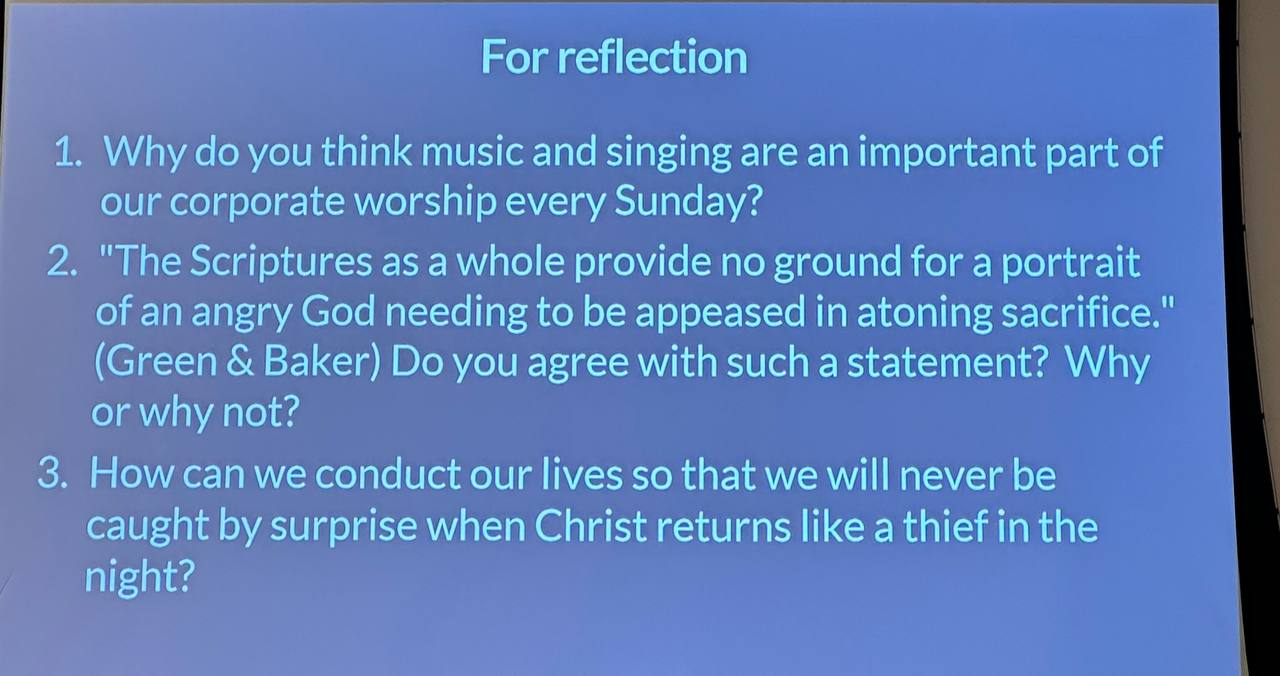
\includegraphics[width=0.8\textwidth, trim={0cm 0cm 0cm 0cm},clip]{Figures/marchSermon4Reflections.jpg}
  %   \includegraphics[width=0.8\textwidth, trim={0cm 0cm 0cm 0cm},clip]{example-image-a}
  %   \caption[]{Reflection questions for this sermon}
  %   \label{}
  % \end{figure}}
\end{itemize}